%----------------南昌工程学院毕业论文LaTeX模板------------------------
%----------------AUTHOR  :  GUANGCHUN-------------------------

\documentclass[UTF8,twoside,AutoFakeBold]{ctexart} % use larger type; default would be 10pt
\usepackage{graphicx}

\usepackage {setspace}%设置正文行间距为1.5倍

\usepackage[a4paper,top=25mm, bottom=20mm, left=25mm, right=20mm]{geometry}%设置页边距
\usepackage{graphicx}%插入图片
\usepackage{booktabs} %美观的表格
\usepackage{amsmath}%数学模式
\usepackage{fancyhdr} %页面布局
%\usepackage{appendix}%附录部分,有的话去掉前面的百分号
\usepackage{titletoc}  %与标题目录有关

\usepackage[square]{natbib}%文献系统
\setmainfont{Times New Roman}

%--------------------------------
%目录样式
%目录页设置
\renewcommand{\contentsname}{\zihao{2}\songti 目\quad 录}
\titlecontents{section}[0em]{\heiti\zihao{4} }{\thecontentslabel\ }{}
{\hspace{.5em}\titlerule*[4pt]{$\cdot$}\contentspage}
\titlecontents{subsection}[2em]{\vspace{0.1\baselineskip}\zihao{-4}}{\thecontentslabel\ }{}
{\hspace{.5em}\titlerule*[4pt]{$\cdot$}\contentspage}
\titlecontents{subsubsection}[4em]{\vspace{0.1\baselineskip}\zihao{-4}}{\thecontentslabel\ }{}
{\hspace{.5em}\titlerule*[4pt]{$\cdot$}\contentspage}

%--------------------------
%三级标题格式

\ctexset {
	section = {
name = {第,章},
number = \chinese{section},
nameformat = \songti \bfseries\zihao{3},
titleformat = \centering\songti \bfseries\zihao{3},
}
}

\ctexset{
	subsection = {
format = \heiti\bfseries\zihao{4},
}
}

\ctexset{
	subsubsection = {
format = \raggedright ,
nameformat = \bfseries\zihao{-4},
titleformat =\songti \bfseries\zihao{-4},
}
}
\setcounter{secnumdepth}{5}
\ctexset{
	paragraph = {	
	name = {,.},
        number=\arabic{paragraph}, 
        format=\indent{}\songti\zihao{-4}
        }
}
\ctexset{
	subparagraph = {
	name = {(,)},
	number = \arabic{subparagraph},
	 format=\songti\zihao{-4}
}
}

%---------------标注样式-----------
	
\newcommand{\upcitep}[1]{\textsuperscript{\textsuperscript{\citep{#1}}}}  
\setcitestyle{numbers}
%---------------------------
%代码设置
\RequirePackage{listings}
\RequirePackage{xcolor}
\definecolor{dkgreen}{rgb}{0,0.6,0}
\definecolor{gray}{rgb}{0.5,0.5,0.5}
\definecolor{mauve}{rgb}{0.58,0,0.82}
\lstset{
	numbers=left,  
	frame=tb,
	aboveskip=3mm,
	belowskip=3mm,
	showstringspaces=false,
	columns=flexible,
	framerule=1pt,
	rulecolor=\color{gray!35},
	backgroundcolor=\color{gray!5},
	basicstyle={\ttfamily},
	numberstyle=\tiny\color{gray},
	keywordstyle=\color{blue},
	commentstyle=\color{dkgreen},
	stringstyle=\color{mauve},
	breaklines=true,
	breakatwhitespace=true,
	tabsize=3,
}
%----------------------------------------------
\begin{document}
%---------------------------------


%-------------------------------
	\begin{titlepage}
	
		\vspace*{0.5cm}
		\centering		
		{\heiti\zihao{-1} 南昌工程学院本(专)毕业设计}
		
		\centering
	{ \songti\zihao{4}
		\vspace*{1.5cm}
		\quad
\includegraphics[width=5.5cm,height=5.5cm]{figures/nit-logo.jpg}\\{}
		
		 \vskip 2cm
	%	 \baselineskip 
		 \makebox[50mm]{~~系~ (院)}
		 \underline{\makebox[75mm][c]{ 这里填写}}\\%院系
		 \vskip 0.9cm
		 \makebox[50mm]{专\qquad 业}
		 \underline{\makebox[75mm][c]{ 这里填写}}\\%专业
		 \vskip 0.9cm
		 \makebox[50mm]{毕业设计(论文)题目}
		 \underline{\makebox[75mm][c]{ 这里填写}}\\%题目
		 \vskip 0.9cm
		 \makebox[50mm]{学生姓名}
		 \underline{\makebox[75mm][c]{ 这里填写}}\\%姓名
		 \vskip 0.9cm
		 \makebox[50mm]{班\qquad  级}
		 \underline{\makebox[75mm][c]{ 这里填写}}\\%班级
		 \vskip 0.9cm
		 \makebox[50mm]{学\qquad 号}
		 \underline{\makebox[75mm][c]{ \LARGE 2016214000}}\\%学号
		 \vskip 0.9cm
		 \makebox[50mm]{指导老师}
		 \underline{\makebox[75mm][c]{ 这里填写}}\\%老师
		 \vskip 0.9cm
		  \makebox[50mm]{完成日期}
		 \underline{\makebox[75mm][c]{ 这里填写}}\\%日期
		 \vskip 1cm
		 \LARGE \heiti{\number \year }~年~\heiti{\number\month}~月~\heiti{\number\day}~日	
	}	 
	\end{titlepage}
%--------------------------------------------------------
%论文题目
\newpage\thispagestyle{empty}	
		\rightline{\quad
\includegraphics[width=5cm,height=1cm]{figures/nit-title.jpg}}
	\vskip 2cm
	\centering

         {\songti  \bfseries \zihao{2} 基于实体建模的数控仿真系统环境的开发  } %标题
         \vskip 0.5cm
        \rightline {\songti \zihao{-2} 小标题}%如果需要小标题的话,没有需要请注释
        \vskip 2.5cm

        { \bfseries \Large The development of Environment for NC Simulation system  based on the solid modelling}%英文标题
        \vskip 13cm
        \begin{flushleft}
        \songti\zihao{4}
        总计\makebox[50mm]{毕业设计(论文)}  \underline{\makebox[25mm][c]{ X}} 页\\
       \quad \quad \makebox[50mm]{表\qquad \quad \qquad 格}  \underline{\makebox[25mm][c]{ X}} 个\\
        \quad \quad \makebox[50mm]{插\qquad \quad\qquad 图}  \underline{\makebox[25mm][c]{ X}}幅\\
        \end{flushleft}
        

%\endtitlepage
%-----------------------------------------	

\newpage\thispagestyle{plain}
\pagenumbering{Roman} %页码采用罗马数字
\renewcommand{\abstractname}{\songti \zihao{3}摘~要}
\addcontentsline{toc}{section}{摘要}
\begin{abstract}
\songti \zihao{-4}
\setlength {\parindent }{2 em}
\par 本文首先对数控加工动态仿真技术的定义、意义、研究重点、研究状况进行了介绍;并介绍了可用于开发数控仿真系统的实体造型平台——ACIS,包括ACIS的开发接口、数据结构、主要功能与特色以及在数控仿真系统开发中的应用;然后通过简要介绍数控加工的一些相关知识,引出了数控仿真系统加工环境的定义与该模块的实现方法;最后讲述了帮助文件的制作以及该系统帮助文件的结构。

\addtolength {\parskip }{16pt} \songti \zihao{5}{\bfseries{关键词:}}数控加工 ~ 数控仿真 ~ 加工环境~ 帮助文件

\end{abstract}


%------------------------------------------------------
\newpage\thispagestyle{plain}

\renewcommand\abstractname{\Large Abstract}
\addcontentsline{toc}{section}{ABSTRACT}
\begin{abstract}
\large
\par First, the definition, significance, research emphases and status of NC machining verification technology are introduced in this paper. Then the platform—ACIS for the development of verification system, including its development interface, data structure, main functions, features and the application in the system is introduced. And, we indicate in brief the correlative knowledge of NC machining and then discuss the definition of the machining environment of NC machining verification system as well as the way that the module has been developed. Finally, we describe how to make Help Files and the structure of the Help Files in the system.

\addtolength {\parskip }{16pt}    \large{\bfseries{key words:}} NC machining; NC verification; Machining environment; Help Files

\end{abstract}

%-------------------------------------------------
%生成目录
\newpage
\tableofcontents\thispagestyle{empty}

\setcounter {tocdepth}{3}

\renewcommand{\thefigure}{\arabic{section}-\arabic{figure}}  %设置图片标题样式
\renewcommand{\thetable}{\arabic{section}-\arabic{table}}  %设置表格标题样式
\renewcommand{\theequation}{\arabic{section}-\arabic{equation}} %设置公式右边注释样式

%------------------------------------------------

\pagestyle{fancy}
\fancyhf{}
\fancyhead[CO]{\songti \zihao{-5}南昌工程学院本(专)科毕业设计(论文) }  %奇数页页眉设置
\fancyhead[CE]{\songti \zihao{-5}\rightmark}   %偶数页页眉设置

\renewcommand\sectionmark [1]{\markboth  {}{第 \thesection 章 : #1}}
\cfoot{\thepage}

%-------------------------------
\newpage
\pagenumbering{arabic}

\raggedright
\setlength {\parindent }{2 em}

\onehalfspacing %正文1.5倍间距
\songti \zihao{-4} %正文采用宋体小四号

\section{一级标题三号宋体加粗居中}   
\subsection{二级标题四号黑体加粗居左}
\subsubsection{三级标题小四号宋体加粗居左}
\par  正文部分用小四号字。……

%---------------------------------
\newpage
\section{网站导航概述}
\subsection{网站导航技术的概念(二级标题四号黑体加粗居左,前后0.5行)}
\par 据参考文献 \citep{Naidu1989Evaluation}(参考文献标注式样之一),所谓网站导航就是针对站点的信息结构,提供组织和导航系统的菜单机制,帮助用户查找信息,从而优化用户体验。网站导航学科要涉及到:传统结构学、管理科学、UI设计学、实用科学等。(正文首行缩进两个汉字符,宋体小四号字,1.5倍行距。)

\subsection{如何设计Web站点的导航}
\par 当开始讨论“网站导航UI设计”,大多会立即与动态脚本,图形,视觉效果设计等等联想起来。这些的确是UI设计中不可忽视的元素。然而一个网站的核心设计所面临的最大挑战是围绕着“信息管理功能”的,并非仅仅是外观视觉。\\

\subsubsection{Web站点导航的分类(三级标题小四号宋体加粗居左,前后0.5行)}
\par Web站点用户导航都包括哪些?在站点中一个多样化的用户导航设计将使得站点的易用性尽可能地提高。根据Web站点导航的目的,可以将导航分为以下几种:\upcitep{Rohden2012Turbine}(参考文献标注式样之二)
\paragraph{核心导航(Core Navigation)(四级标题首行缩进两个字符,宋体小四号字。)} 
\par 核心导航是Web站点主体信息的体现。它将一个Web站点所提供的信息进行了最基本的归类,并以导航条的形式页面的正上方,这样可以清楚地被访问者发现。核心导航应该被一个网站里的每个页面所包含。
\subparagraph{命名一个片段(五级标题首行缩进两个字符,宋体小四号字。)}
\par 首先必须确定并命名文文档中的一段需要链接到的文字,使用锚点(anchor)<a>标记,并设定属性NAME的值。如
<a name="part1">链接到:第一章 网站导航设计概述</a>(程序段五号宋体居左,1倍行距)
有以下几种方法使一个Web文档中的元素应用CSS。但这种情况也应该尽量避免,最好还是把HTML和CSS用单独的档存放\footnote{在外链的CSS中没有<style>标签。}。(随文脚注式样)
\paragraph{地区导航(Geographic Navigation)}
\par 当网站划分为多个地区(可以是国家,也可以是一个国家内不同区域)性的子站点\citep{宫琳2017基于专利信息的产品方案竞争力评价方法} ,需要地区导航。

%---------------------------------
\newpage
\begin {figure}[htbp]
\centering
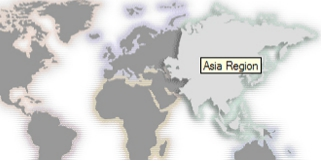
\includegraphics {figures/figure-example.jpg}
\caption{\songti \zihao{5}地区导航(图题放在图下,按章顺序编号。五号宋体居中。)}
\label{fig:figure-example}
\end{figure}

\subsubsection{网站导航的表现形式}
\par 网站导航根据不同Web站点的需要可以布置为多种表现形式,其中常见的表现形式如表\ref{tab:1}所示。
\begin{table}[htbp]
\centering
\caption{\heiti \zihao{5}网站导航的表现形式}
\label{tab:1}
\begin{tabular}{llll}
	\toprule
	类型  &名称  &  英文名  & 特点  \\
	\midrule
	1  &    面包屑  &  breadcrumb trail & 简单 \\
	2  &  下拉导航菜单  & Drop-Down Navigation Menus  & 常用 \\
	3  &   弹出式导航菜单  &  Pop-Up Navigation Menus &  容量大 \\
	4  &  树形导航  &  Tree-View Navigation & 可操控复杂流程 \\
	\bottomrule
\end{tabular}
\end{table}
	
\par 对x,$\theta$求二阶混合偏导数得: \\
\begin{equation}
\centering
 \frac{\partial u(x,\nu(x),\theta)}{\partial x} = (1-\omega)\bar \nu^{'}(x)-\frac{\omega L_1}{\theta}
\end{equation}
%---------------------------------------------
\newpage

\section{程序代码}
\begin{lstlisting}[language=C++,escapeinside=``]
#include<iostream>
using namespace std;
int main
{
	cout<<"Hello world!"<<endl;//`输出`
	return 0;
}
\end{lstlisting}

%\begin{appendices}
%\end{appendices}
%----------------------------------------------
%----------------------
\newpage
\bibliographystyle{plainnat}
\bibliography{bib-example}
\addcontentsline{toc}{section}{参考文献} %添加到目录

%\backmatter %在此命令后恢复成罗马数字页码
\end{document}
